\subsection{Electron Drifting}
\label{sec:elec}
The dependence of the electron drift velocity $\mathbf{v}_{e}$ on the applied electric field $\mathbf{E}$ is taken to be
\begin{equation}
  \label{eq:ed}
  \mathbf{v}_{e} = \mathcal{A}(|\mathbf{E}|) \sum_{j} \frac{n_{j}}{n}     \frac{\gamma_{j}\mathbf{E_{0}}}     {\sqrt{\mathbf{E_{0}}\gamma_{j}\mathbf{E_{0}}}},  \mbox{ with }     j=1,2,3,4
\end{equation}
where $\mathcal{A}$ is a function of the magnitude of the electric field and temperature, the value of $\mathcal{A}$ must be negative because electrons drift to the opposite direction of the electric field; $\mathbf{E_{0}}$ is the normalized electric field vector; $n_{j}/n$ is the fraction  of the carriers (in this case, electrons) in the $j$-th valley, $\gamma_{j}$ is the effective mass tensor for the $j$-th valley. In general the tensor $j$-th is given in terms of the rotation matrices $R_{i}$, responsible for aligning the $i$-th $\langle 111 \rangle$ axis with the Y-axis of the lab system, by
\begin{equation}
  \label{eq:gammas}
  \gamma_{j} = R_{j}^{T}\gamma_{0}R_{j}, \mbox{ with } \gamma_{0}   \equiv \left(
    \begin{array}{ccc}
      m_{t}^{-1} & 0 & 0 \\
      0 & m_{l}^{-1} & 0 \\
      0 & 0 & m_{t}^{-1}
    \end{array} \right),
\end{equation}
where $m_{t} = 1.64m_{e}, m_{l} = 0.0819m_{e}$ with $m_{e}$ denoting the free electron mass, and the rotation matrix $R_{j} = R_{x^{\prime}}(\arccos(\sqrt{2/3}))R_{z}((j-1)\pi/2)$.

\begin{figure}[tbhp]
  \centering
  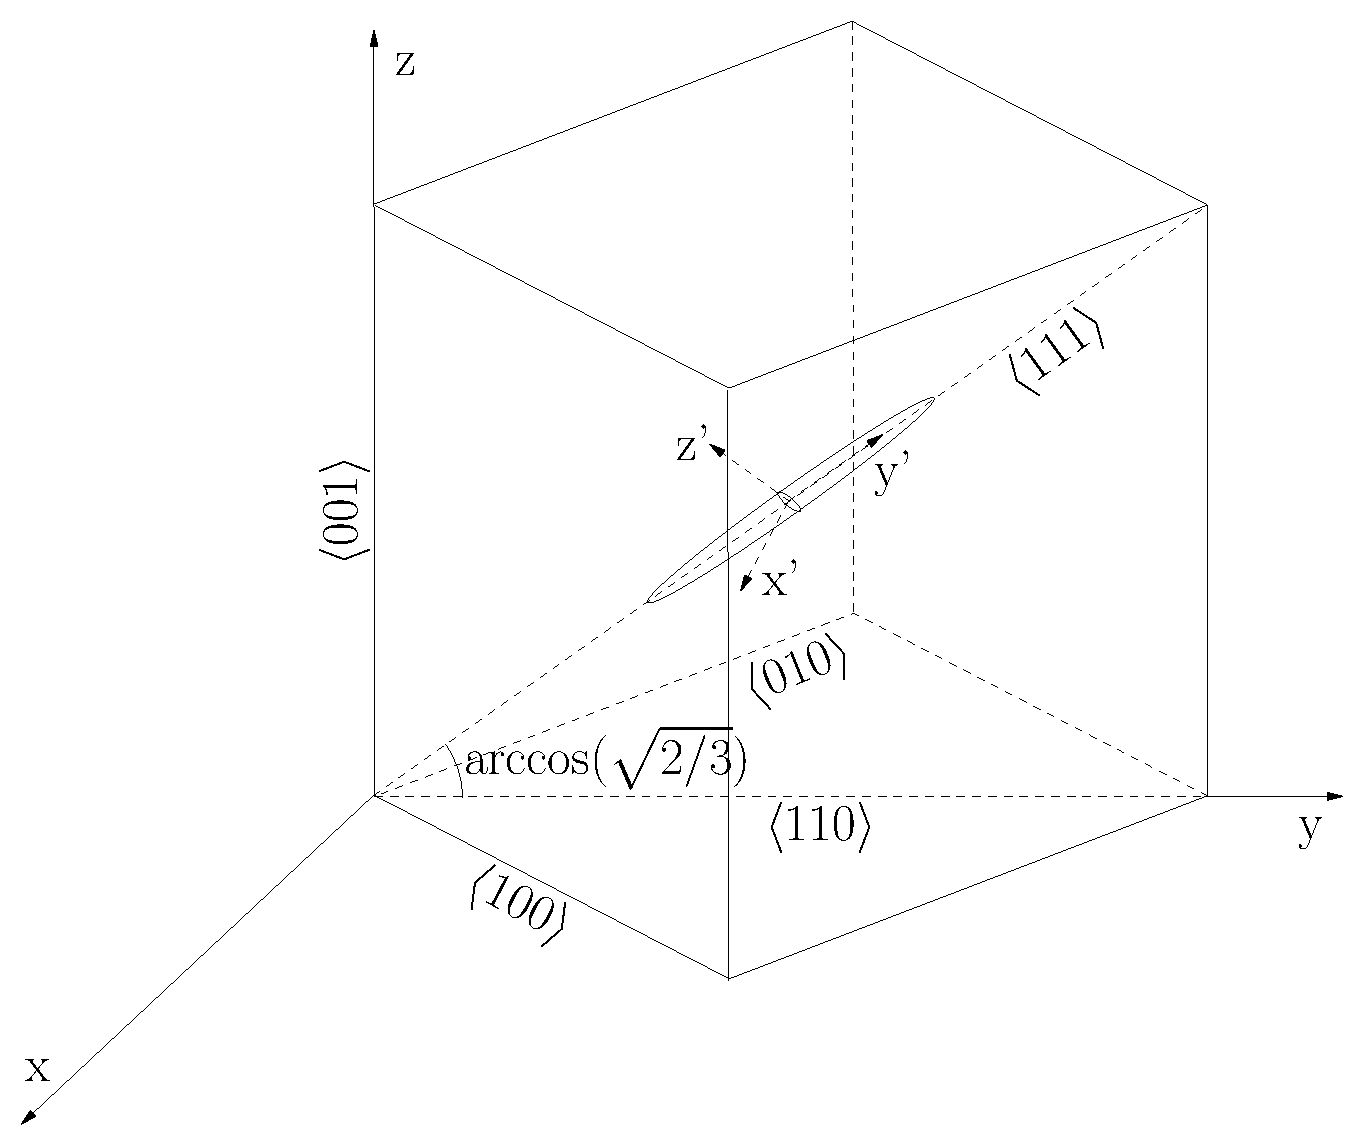
\includegraphics[width=0.6\textwidth]{axes.eps}  
  \caption{Orientations of the crystal axes and valleys in the lab coordinate system XYZ.}
  \label{fig:axes}
\end{figure}

For an experimental determination of the repopulation amplitude, the deviation from a uniform population distribution $n_{e}/n$ (1/4 for germanium) is assumed to vary with the electric field weighted by the factor $\mathcal{R}$:
\begin{equation}
  \label{eq:nion}
  \frac{n_{j}}{n} = \mathcal{R(|\mathbf{E}|)}   \left[         \frac{\sqrt{\mathbf{E_{0}}\gamma_{j}\mathbf{E_{0}}}}
    {\sum_{i}\sqrt{\mathbf{E_{0}}\gamma_{i}\mathbf{E_{0}}}} -               \frac{n_{e}}{n} \right] + \frac{n_{e}}{n},  \mbox{ with }           i=1,2,3,4
\end{equation}



\subsection{Hole Drifting}
\label{sec:hole}
%%% Local Variables:
%%% mode:latex
%%% TeX-master: "GSTR-08-M00x"
%%% End:
